\documentclass[11pt,letterpaper]{article}
\usepackage[T1]{fontenc}
\usepackage[utf8]{inputenc}
\usepackage{lmodern,microtype}
\usepackage[margin=1in]{geometry}
\usepackage{amsmath,amssymb,amsthm,mathtools}
\usepackage{booktabs,longtable,array,enumitem,xcolor}
\newcolumntype{P}[1]{>{\raggedright\arraybackslash}p{#1}}
\usepackage{graphicx,tikz}
\usetikzlibrary{arrows.meta,positioning}
\usepackage{listings}
\usepackage[breaklinks=true,colorlinks=true,linkcolor=blue!45!black,citecolor=teal!65!black,urlcolor=blue!55!black]{hyperref}
\usepackage{fancyhdr}
\usepackage{needspace}
\definecolor{navy}{RGB}{24,48,77}
\definecolor{teal}{RGB}{13,111,116}
\definecolor{lightgray}{RGB}{246,247,249}
\pagestyle{fancy}
\fancyhf{}
\fancyhead[L]{\small Faster algebra and certified knot obstructions}
\fancyhead[R]{\small ProveIt research continuation}
\fancyfoot[C]{\thepage}
\setlength{\headheight}{14pt}
\setlength{\emergencystretch}{3em}
\setlist{topsep=4pt,itemsep=3pt}
\newtheorem{theorem}{Theorem}[section]
\newtheorem{proposition}[theorem]{Proposition}
\newtheorem{lemma}[theorem]{Lemma}
\newtheorem{corollary}[theorem]{Corollary}
\theoremstyle{definition}
\newtheorem{definition}[theorem]{Definition}
\newtheorem{example}[theorem]{Example}
\newtheorem{question}[theorem]{Question}
\theoremstyle{remark}
\newtheorem{remark}[theorem]{Remark}
\newcommand{\F}{\mathbb F_2}
\newcommand{\N}{\mathbb N}
\newcommand{\Kh}{\operatorname{Kh}}
\newcommand{\End}{\operatorname{End}}
\newcommand{\Hom}{\operatorname{Hom}}
\newcommand{\Inn}{\operatorname{Inn}}
\newcommand{\supp}{\operatorname{supp}}
\newcommand{\poly}{\operatorname{poly}}
\newcommand{\bits}{\operatorname{bits}}
\newcommand{\rank}{\operatorname{rank}}
\newcommand{\ceil}[1]{\left\lceil#1\right\rceil}
\newcommand{\floor}[1]{\left\lfloor#1\right\rfloor}
\lstset{basicstyle=\ttfamily\small,backgroundcolor=\color{lightgray},breaklines=true,columns=fullflexible,keepspaces=true,frame=single,rulecolor=\color{gray!25},showstringspaces=false}
\title{\color{navy}\bfseries Faster Cobordism Composition and Certified Finite Quotient Filters for Unknot Recognition}
\author{Research continuation for Vladimir Reshetnikov's ProveIt project}
\date{8 October 2026}
\begin{document}
\maketitle
\begin{abstract}
We improve two concrete parts of the ProveIt unknot-recognition program.
First, we factor every genus-zero
composition in its characteristic-two dotted-cobordism algebra into variable
identification, multiplication in a squarefree algebra, and an output map.
Ranked subset convolution then replaces a dense loop over as many as
$4^m$ pairs of terms by a coefficient algorithm using
$\poly(m)2^m$ bit operations, where $2m$ is the number of exposed endpoints.
The implementation also avoids a hidden extra exponential factor from
repeated updates of large packed integers. Recovering the discarded
quantum grading sharpens the earlier component-type exponent from
$b^2 2^m$ to $b^2\binom{m}{\floor{m/2}}$ for components with at most
$b$ objects. Second, we implement bounded
$A_5$ searches that return explicit permutation-valued knottedness witnesses
and have a separate verifier. A constructive Wirtinger seed plan gives an
exhaustive search bound in terms of the number of seeds.

The article supplies complete proofs, differential and certificate checks,
paired measurements, an integration patch, and research priorities. We also
prove a useful limitation: for every prime $p>3$, the determinant-one torus
knot $T(3,p)$ has no nonconstant coloring by any finite quandle of size less
than $p$. The standard diagram has $2p$ crossings. This is a limitation of
finite palettes, not of the complete recognition pipeline. The improved
local algebra is near its explicit coefficient-table size; the remaining
global problem is controlling the chain complexes or replacing them with
constructively bounded geometric data. A general quasi-polynomial running
time is not established here.
\end{abstract}
\thispagestyle{empty}
\clearpage
\tableofcontents
\clearpage
\section{Outcome, scope, and relation to earlier work}
\label{sec:overview}

The project already has an exact recognizer. Its unsolved performance
problem is a worst-case complexity problem, not a missing correctness
criterion. In particular, the Khovanov backend decides triviality from the
rank of reduced homology over $\F$~\cite{kronheimer,shumakovitch}.
Kronheimer and Mrowka prove that a nontrivial knot has reduced rational
Khovanov rank greater than one. The universal coefficient theorem makes
the total reduced rank over $\F$ at least that rational rank, whereas the
unknot has reduced rank one. Over $\F$, unreduced homology is the direct
sum of two quantum-shifted copies of reduced homology, so dividing its
total rank by two gives the same decision criterion.
The present continuation concentrates
on making an expensive algebraic primitive substantially cheaper and on
providing a complementary, independently checkable obstruction.

\subsection{What this continuation contributes}

There are five main contributions. The first is an exact factorization of
the existing compiled cobordism plans. It applies to arbitrary morphisms in
the implemented algebra, including dense ones; it does not assume that a
particular knot family creates them. The second is an implementation whose
coefficient manipulation respects a bit-cost model. The distinction is
essential because a morphism with $m$ possible dots is a $2^m$-bit integer,
not an $m$-bit integer. The third recovers a grading invariant and uses it
to sharpen the sufficient parameter regime for exact component sharing.
The fourth is a finite-group certificate backend with
explicit construction and verification semantics. The fifth is a precise
separation of the local improvement from the global hypotheses that would
be needed for a quasi-polynomial recognizer.

\begin{center}
\small
\begin{tabular}{P{.26\linewidth}P{.40\linewidth}P{.23\linewidth}}
\toprule
Result & Mathematical content & Status \\
\midrule
Cobordism factorization & Input contraction, squarefree multiplication,
output reconstruction & Proved and implemented \\
Dense coefficient bound & $\poly(m)2^m$ bit cost for $2m$ endpoints &
Unconditional local bound \\
Homogeneous type count & $b^2\binom{m}{\floor{m/2}}$ in the sufficient
component-sharing exponent & Proved; conditional global use \\
Finite-group certificates & Noncyclic $A_5$ representation implies knottedness &
Proved; separate verifier \\
Wirtinger seed search & Exhaustive search with $q^{b-1}$ assignments for a
checked $b$-seed plan & Parameterized bound \\
Palette obstruction & $T(3,p)$ needs at least $p$ quandle colors &
Proved; no priority claim \\
Full quasi-polynomial recognition & Requires bounds on surviving data or a
constructive geometric hierarchy & Unresolved \\
\bottomrule
\end{tabular}
\end{center}

The subset-convolution algorithm itself is due to Bj\"orklund, Husfeldt,
Kaski, and Koivisto~\cite{bhkk}. Quandle coloring, normalization of one
meridian color, and the use of non-affine targets after a trivial Alexander
polynomial also precede this work~\cite{clark,fish}. Our claims concern the
factorization and implementation for this repository, the accompanying
bit-cost audit, the concrete certificate backend, and the deductions proved
below. We make no claim to have invented these underlying theories.

\Needspace{12\baselineskip}
\subsection{Sources and pinned baseline}

The computational baseline is the \texttt{fast/} subtree at ProveIt commit
\begin{center}
\texttt{ca61a1a5f967999d778d6efd7c882e77a2eb379d}.
\end{center}
Its tree identifier is
\texttt{b99a666269f660d932fc82ac8d1f29d3ae42231f}. The baseline source is
included in the archive so that comparisons do not depend on later
repository changes. Forty-one baseline unit tests passed in this
environment before modification.

The audit also read the structural-compression report now stored under
\texttt{reports/07}, and two recent continuation archives:
\nolinkurl{unknot_progress_20261007.zip} and
\nolinkurl{unknot_recognition_progress.zip}. These contain, respectively,
improved interlacement factorization, sparse Alexander elimination and a
pointed scanner; and an exact three-braid backend, Markov descent, and a
study of intrinsic scanner multiplicities. Report 07 contributes
homogeneous Seifert-graph certificates and exact component sharing. Those
results are antecedents, not results newly established by the present
measurements. The integration patch is against the pinned \texttt{fast/}
baseline, not an untested merge of every recent branch.

We inspected the README and manuscript catalogue of
\texttt{openai/math} at commit
\begin{center}
\texttt{adc7f1241b42e322a6451854ab7e4b4c146bf78a}.
\end{center}
The catalogue search did
not identify a directly applicable unknot-recognition theorem. No theorem
in the present argument is imported from that collection, and this limited
catalogue audit is not represented as a verification of its manuscripts.
The source record includes both repository revisions~\cite{proveit,openai}
and the relevant
primary literature.

\subsection{The precise quasi-polynomial target}

We use the standard broad terminology
\[
 T(n)=\exp\bigl((\log(n+2))^{O(1)}\bigr)
\]
for quasi-polynomial time. The repository's explicit objective
$n^{O(\log n)}$ is the stronger, particular scale
$\exp(O((\log n)^2))$.

Lackenby's detailed 2021 handout states an announced bound
$2^{O((\log n)^3)}$, equivalently $n^{O((\log n)^2)}$~\cite{lackenbytalk}.
His July 2026 preprint develops incompressible surfaces, boundary patterns,
and certifiable hierarchies~\cite{lackenby2026}. Its Section 9 separates
step counts from running time; several operations do not yet have the
precision needed for that cost analysis. The useful displayed search bound
is $L(g+1)^L$ in terms of hierarchy length $L$ and pattern complexity $g$.
The introduction reserves further speed-up for future work. Neither an
efficiently checkable hierarchy nor that parameterized visit count is, by
itself, a construction in the desired time bound.

Our end-to-end discussion therefore has two distinct questions. How much
does each local algebraic operation cost on the data actually present?
How large can the data become, and can the required data be constructed?
The first receives an unconditional improvement here. The second remains
the central research problem.

\subsection{Conventions and trust boundary}

Inputs are validated planar diagrams of a single knot. A diagram has $n$
crossings and integer edge labels; labels can be renumbered to have
$O(\log(n+2))$ bits. During a scan, $w=2m$ denotes the number of exposed
endpoints. Each object is a loopless matching on those endpoints, with a
homological degree. Closed circles are delooped. All cobordism
coefficients in this continuation are in $\F$; the integer or odd-prime
coefficient theories require additional sign and coefficient analysis.

We distinguish three kinds of evidence. A proof justifies an algorithm on
all inputs satisfying its hypotheses. An exhaustive finite test checks a
specified finite domain. A benchmark reports a measured execution on a
specified host and input. None substitutes for either of the others.
The accompanying proofs have not been formally checked in Lean, and the
computational checks are stated at their actual scope.

\section{A factorization of the implemented cobordism algebra}
\label{sec:algebra}

\subsection{Coefficient tables and gluing plans}

Let $a,b$ be loopless matchings on $2m$ exposed endpoints. Gluing $a$ to
the reflected $b$ produces $k(a,b)$ circles, where $k(a,b)\leq m$. A basis
of $\Hom(a,b)$ is indexed by the subsets of those circles: a selected circle
carries a dot. Thus a morphism is a coefficient table of length
$2^{k(a,b)}$. The program stores this table as an integer
\[
 f=\sum_{S\subseteq[k(a,b)]} f_S\,2^{\operatorname{mask}(S)},
 \qquad f_S\in\{0,1\}.
\]
The exponent in this formula is a subset mask. In particular, the bit
length of the packed integer is exponential in the number of circles.

For a composition
\[
 a\xrightarrow{f}b\xrightarrow{g}c
\]
write $k_L=k(a,b)$, $k_R=k(b,c)$, and $k_O=k(a,c)$. The existing geometry
compiler decomposes the glued surface into connected components. For a
genus-zero component $s$ it records
\[
 (L_s,R_s,B_s,e_s),
\]
where $L_s$, $R_s$, and $B_s$ are the sets of left input, right input, and
output circles belonging to the component, and $e_s$ counts any already
present dots. In ordinary composition $e_s=0$. The generalized notation is
also useful for crossing-transfer plans with cups and caps.

Within each of the three families the sets are pairwise disjoint and cover
the corresponding circle set. Empty sets are allowed. A positive-genus
component gives zero in this characteristic-two theory: the handle
operator is comultiplication followed by multiplication, and equals
multiplication by $2x=0$. Two dots on one component also give zero. These
are exactly the relations used by the baseline~\cite{barnatan,proveit}.

The old composition routine enumerates every supported pair $(S,T)$,
checks the number of dots on every component, and reconstructs its output.
Even when most pairs vanish, it has already visited them. If $a=b=c$ has
$m$ arcs, each input can have $2^m$ supported monomials, producing a
$\Theta(4^m)$ term-pair loop.

\subsection{Squarefree algebras and contraction}

For a nonnegative integer $r$ let
\[
 R_r=\F[y_1,\ldots,y_r]/(y_1^2,\ldots,y_r^2).
\]
Write $y_S=\prod_{s\in S}y_s$. Then
\begin{equation}
 y_Sy_T=
 \begin{cases}
 y_{S\cup T},&S\cap T=\varnothing,\\
 0,&S\cap T\ne\varnothing.
 \end{cases}
 \label{eq:squarefree}
\end{equation}
The dot algebra $A=\F[x]/(x^2)$ is $R_1$.

Suppose a genus-zero plan has $r$ connected components. Define
\[
 \rho_L:R_{k_L}\longrightarrow R_r,
 \qquad x_j\longmapsto y_s\quad(j\in L_s),
\]
and similarly define $\rho_R$ using the sets $R_s$. These are well-defined
algebra homomorphisms because every image variable squares to zero.

\begin{lemma}[Input contraction]
\label{lem:contraction}
If an input monomial selects two circles belonging to one component,
its image under $\rho_L$ is zero. Otherwise its image selects exactly the
components containing a chosen circle. Coefficients of input monomials
with the same image add modulo two.
\end{lemma}
\begin{proof}
Substitute the defining image of every variable into the monomial. A
repeated component introduces a factor $y_s^2$. If there is no repetition,
the product is the squarefree monomial on the selected component set.
Linearity gives the coefficient assertion.
\end{proof}

This contraction can eliminate a large fraction of a dense input before
the two morphisms are multiplied. It also combines distinct monomials by
parity, which cannot be reproduced merely by forgetting duplicate
component labels in a list of supported terms.

\subsection{The output map}

For a component with $b$ output circles, define a linear map
$T_b:A\to A^{\otimes b}$ by
\begin{align}
 T_0(1)&=0, &T_0(x)&=1,\label{eq:trace}\\
 T_b(1)&=\sum_{j=1}^{b}\prod_{\ell\ne j}z_\ell,
 &T_b(x)&=\prod_{\ell=1}^{b}z_\ell\qquad(b\geq1).
 \label{eq:comultiplication}
\end{align}
The empty product is one. Formula~\eqref{eq:comultiplication} follows by
iterating $\Delta(1)=1\otimes x+x\otimes1$ and
$\Delta(x)=x\otimes x$. The output variable sets belonging to distinct
components are disjoint.

Let $T=\bigotimes_{s=1}^{r}T_{|B_s|}$, with output variables placed at the
indices specified by the $B_s$. Multiplication by $y_s^{e_s}$ accounts for
the dots already supplied by the plan.

\begin{theorem}[Exact composition factorization]
\label{thm:factorization}
For any genus-zero compiled plan with the partition properties above,
the baseline composition is exactly
\begin{equation}
 g\circ f
 =T\left(\rho_L(f)\rho_R(g)\prod_{s=1}^{r}y_s^{e_s}\right).
 \label{eq:factorization}
\end{equation}
If the plan contains a positive-genus component, both sides are understood
to be zero. If any $e_s\geq2$, the result is zero.
\end{theorem}
\begin{proof}
Both constructions are bilinear in $f$ and $g$, so it suffices to take
monomial inputs. For each component, the total number of dots is
\[
 d_s=|S\cap L_s|+|T\cap R_s|+e_s.
\]
The contractions and multiplication in $R_r$ kill the monomial if some
$d_s\geq2$. This is the two-dot relation used by the baseline. Otherwise
the component is undotted or singly dotted. If it has no output circle,
the counit~\eqref{eq:trace} kills precisely the undotted case. If it has
output circles,~\eqref{eq:comultiplication} is precisely the baseline's
sum over leaving one output circle undotted, or its single all-dotted
term. Finally, different components use disjoint output variables, so their
contributions multiply without any additional identification. These cases
exhaust the baseline evaluation of the monomial pair. Extend by
bilinearity.
\end{proof}

\begin{center}
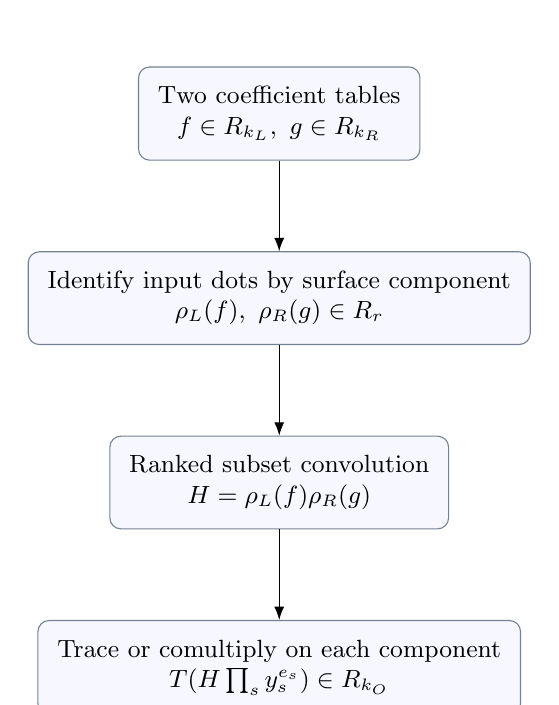
\begin{tikzpicture}[node distance=1.15cm,>=Latex,
 every node/.style={font=\small,align=center},
 box/.style={draw=navy!60,rounded corners,fill=blue!3,inner sep=7pt}]
\node[box] (inputs) {Two coefficient tables\\$f\in R_{k_L},\ g\in R_{k_R}$};
\node[box,below=of inputs] (contract) {Identify input dots by surface component\\$\rho_L(f),\ \rho_R(g)\in R_r$};
\node[box,below=of contract] (multiply) {Ranked subset convolution\\$H=\rho_L(f)\rho_R(g)$};
\node[box,below=of multiply] (output) {Trace or comultiply on each component\\$T(H\prod_s y_s^{e_s})\in R_{k_O}$};
\draw[->] (inputs)--(contract);
\draw[->] (contract)--(multiply);
\draw[->] (multiply)--(output);
\end{tikzpicture}
\end{center}

\subsection{Output reconstruction without exponential repeated expansion}

Expanding~\eqref{eq:comultiplication} separately for every supported
component monomial can itself repeat a large amount of work. There is a
better way: determine the one input coefficient, if any, that contributes
to a given output coefficient.

Fix an output subset $U\subseteq[k_O]$. For each component define the
required final dot count
\[
 d_s(U)=
 \begin{cases}
 1,&B_s=\varnothing,\\
 1,&B_s\subseteq U,\\
 0,&|B_s\setminus U|=1,\\
 \text{invalid},&|B_s\setminus U|\geq2.
 \end{cases}
\]
The first case is the trace condition, not a statement that a closed
component has an output dot. Subtract the fixed extra-dot count and put
$v_s(U)=d_s(U)-e_s$. If any requirement is invalid or any $v_s(U)$ lies
outside $\{0,1\}$, set the output coefficient to zero. Otherwise let
$D(U)=\{s:v_s(U)=1\}$.

\begin{lemma}[Unique coefficient lookup]
\label{lem:output}
Writing $H=\rho_L(f)\rho_R(g)$, the coefficient of $z_U$ in
\eqref{eq:factorization} is $H_{D(U)}$ when the requirements are valid, and
zero otherwise.
\end{lemma}
\begin{proof}
For a nonempty output block, a singly dotted input gives exactly the
all-dotted monomial. An undotted input gives each monomial with exactly
one missing dot, once. These alternatives have disjoint supports. For an
empty block the trace requires a singly dotted input. Thus $U$ uniquely
determines the final dot count on every component. Subtracting the dots
already supplied determines the unique contributing component monomial.
There is no multiplicity coefficient to compute.
\end{proof}

\begin{example}[Why dot identification requires parity]
Let two left circles belong to one component. The left morphism
$x_1+x_2+x_1x_2$ contracts to $y+y+0=0$. Treating its two linear terms as
one supported term would give the wrong result. Conversely, two inputs
each containing a dot on the same component multiply to zero even if their
original circle indices are different.
\end{example}

\begin{example}[Closed components and extra dots]
A closed component with no extra dot requires the coefficient of $y$;
with one extra dot it requires the coefficient of $1$. With two extra
dots it annihilates the plan. For a one-circle output, the map is the
identity on $A$ before extra dots: an undotted component outputs $1$,
not $x$.
\end{example}

\section{Ranked subset convolution and the coefficient bound}
\label{sec:convolution}

\subsection{The multiplication problem}

By~\eqref{eq:squarefree}, multiplying two coefficient arrays $F,G$ in
$R_r$ means computing
\begin{equation}
 H_S=\sum_{A\subseteq S}F_A G_{S\setminus A}.
 \label{eq:subsetconvolution}
\end{equation}
Enumerating all ordered disjoint pairs takes $3^r$ iterations. The
baseline's general-purpose pair loop can do even more work by visiting
overlapping pairs before rejecting them. Ranked subset convolution computes
all coefficients using $O((r+1)^2 2^r)$ field operations~\cite{bhkk}.
For completeness, the exact characteristic-two specialization used here
has the following short verification.

For every $S\subseteq[r]$ form rank polynomials
\[
 \widehat F_S(t)=\sum_{A\subseteq S}F_A t^{|A|},
 \qquad
 \widehat G_S(t)=\sum_{B\subseteq S}G_B t^{|B|}.
\]
Multiply these polynomials and apply subset M\"obius inversion to the
array indexed by $S$. In characteristic two the M\"obius transform is
the same XOR transform as the zeta transform. Call the resulting polynomial
array $W_S(t)$. Then
\begin{equation}
 H_S=[t^{|S|}]W_S(t).
 \label{eq:rankextraction}
\end{equation}

\begin{proof}[Verification of~\eqref{eq:rankextraction}]
Before inversion, the term $F_A G_B t^{|A|+|B|}$ occurs at every index
containing $A\cup B$. After inversion it occurs only at index
$S=A\cup B$. Requiring its degree to equal $|S|$ gives
$|A|+|B|=|A\cup B|$, which is equivalent to disjointness. Thus the
remaining terms are exactly those of~\eqref{eq:subsetconvolution}.
\end{proof}

Only ranks $0,\ldots,r$ are needed. Higher terms may be discarded before
the inverse transform because that transform does not mix polynomial
degrees. An unranked zeta transform would compute union convolution and
would incorrectly replace $x\cdot x=0$ by $x\cdot x=x$.

\subsection{Why the number of surface components stays small}

\begin{lemma}[Component count for matching composition]
\label{lem:components}
For a composition of three matchings on $2m$ endpoints,
\[
 k_L,k_R,k_O\leq m,
 \qquad r\leq\min(k_L,k_R)\leq m.
\]
\end{lemma}
\begin{proof}
Every circle in a pair of matchings uses at least one arc from either
matching, giving the first three bounds. Every left input disc meets at
least one middle-matching arc, and so is glued to a right input disc. The
same argument applies on the right. Consequently each connected glued
component contains at least one left disc and one right disc. Distinct
components contain disjoint input discs, giving the asserted bound on $r$.
\end{proof}

This argument is needed. For an arbitrary abstract list of surface
components with many empty input blocks, $r$ can exceed the three circle
counts. The generic implementation supports such plans but charges for
$2^r$ explicitly; the matching-composition bound is applied only after
Lemma~\ref{lem:components}.

\begin{theorem}[Dense local coefficient complexity]
\label{thm:densecost}
Given a compiled composition plan of matchings on $2m$ endpoints and the
two full coefficient tables over $\F$, the output can be computed in
$\poly(m)2^m$ bit operations and $\poly(m)2^m$ bits of working storage.
The field-operation count of the ranked multiplication is
$O((m+1)^2 2^m)$. The implementation's explicit array and index arithmetic
admits a conservative bound $O((m+1)^3 2^m)$ for the coefficient work in a
random-access bit-cost model. Label manipulation in constructing the plan
adds a polynomial in $m$ and the label bit length.
\end{theorem}
\begin{proof}
For each input, precompute the image of every subset by taking off one
selected variable at a time. Store a sentinel for a repeated component.
This uses $O(2^{k_L}+2^{k_R})$ entries with $O(m)$ bits per entry.
Read each coefficient once, and toggle its contracted coefficient if its
image is valid. Ranked convolution uses arrays of $2^r$ polynomials, each
of at most $r+1$ bits. Its zeta transforms perform $O(r2^r)$ XORs on
$O(r)$-bit words. Naive carryless multiplication of two rank polynomials
takes $O((r+1)^2)$ bit operations, at each of $2^r$ indices.

For every one of $2^{k_O}$ output subsets, inspect its intersection with
each output block and use Lemma~\ref{lem:output}. This uses only integers
of $O(m)$ bits. The input and output full morphisms are converted to and
from byte arrays once. In particular, there is no loop making $2^m$
updates to an integer of $2^m$ bits. Charging conservatively for array
indices and small masks adds at most an additional polynomial factor.
Lemma~\ref{lem:components} bounds all four exponential dimensions by
$2^m$. The stored tables have $O(2^m)$ entries of $O(m)$ bits, together
with the packed inputs and output.
\end{proof}

\begin{remark}[Meaning of the improvement]
The theorem compares complete coefficient operations. The old
$\Theta(4^m)$ statement counts term pairs; it is not an assertion that
the old bit complexity is exactly $\Theta(4^m)$. Its packed-integer
operations can cost more. The new theorem supplies a bit bound for its
own coefficient kernel. On a model that explicitly writes the output
table, the worst-case output size already costs $\Omega(2^m)$, so the
remaining overhead is polynomial in $m$.
\end{remark}

\begin{example}[An explicit dense test family]
In $\End(a)=R_m$, take
\[
 F=\prod_{i=1}^m(1+x_i),\qquad G=F+1.
\]
The two supports have sizes $2^m$ and $2^m-1$. Since every positive-degree
element squares to zero in this commutative characteristic-two algebra,
$F^2=1$ and $FG=F+1$. The baseline nevertheless visits
$2^m(2^m-1)$ pairs. This is a family of valid algebra inputs, not a claim
that the scanner must produce these particular morphisms from knot
diagrams.
\end{example}

\section{Homogeneous entries and a cheaper multiplication path}
\label{sec:homogeneous}

The general dense algorithm works for arbitrary inputs. Genuine scanner
entries have more structure, even though the original implementation does
not retain the quantum grading in its object records.

\Needspace{18\baselineskip}
\begin{samepage}
\begin{proposition}[Recovering the erased grading]
\label{prop:grading}
Assign the initial empty object a shift $q=0$. If a parent object of shift
$q$ is extended by smoothing $i\in\{0,1\}$, and that smoothing creates
$c$ closed circles with delooping label $\ell$, assign its child
\begin{equation}
 q'=q+i+c-2\operatorname{popcount}(\ell).
 \label{eq:qshadow}
\end{equation}
For a nonzero differential entry from object $u$ to object $v$, every
supported monomial with $d$ dots satisfies
\begin{equation}
 k(a_u,a_v)-m-2d+q_v-q_u=0,
 \label{eq:qdegree}
\end{equation}
where $2m$ is the current frontier. The invariant holds before and after
each scalar-unit cancellation. In particular, every nonzero entry is
homogeneous in dot degree, and every cancellable entry between equal
matchings is exactly the identity coefficient $1$.
\end{proposition}
\end{samepage}
\begin{proof}
A canonical cobordism with $k$ discs and $d$ dots has degree
$k-m-2d$, obtained by subtracting the arc normalization $m$ from its
Euler degree. A crossing saddle has degree $-1$, compensated by the
smoothing shift $i$. A delooping label on $c$ circles has degree
$c-2\operatorname{popcount}(\ell)$. Its inclusion contributes this
degree and its projection the negative degree. Consequently the source
and target delooping contributions and the smoothing shift cancel exactly
as in~\eqref{eq:qshadow}. This proves~\eqref{eq:qdegree} inductively
through a crossing extension and delooping.

For completeness, composition respects the claimed degree. In a
genus-zero plan without extra dots, Euler characteristic gives
$2r=k_L+k_R+k_O-m$. Every nonzero output term has
$d_O=k_O-r+d_L+d_R$ dots; a closed component obeys the same formula
because its required input dot contributes $-1+1=0$. Substitution shows
\[
 k_O-m-2d_O=(k_L-m-2d_L)+(k_R-m-2d_R).
\]
Thus map degrees add. A homogeneous entry with equal source and target
matching has monomial degrees $-2d$. If its constant term is nonzero,
homogeneity forces $d=0$ for every term, and there is just one such
monomial. It is therefore $1$, and the two object shifts are equal.
The Schur-complement correction in a cancellation is a composition of
homogeneous maps through this identity. Its source and target shifts
telescope, so it has the same degree as the entry to which it is added.
This proves preservation by cancellation.
\end{proof}

This is a recovered grading of the actual ungraded computation. It does
not rely on guessing a degree from the integer encoding. The grading
audit checks every entry of its pre- and post-elimination stage complexes;
transient Schur-complement entries inside a cancellation sequence are
covered by the proof. The implementation still supports arbitrary ungraded
morphisms, so it retains the general ranked-convolution fallback.

\begin{theorem}[Homogeneous convolution]
\label{thm:homogeneous}
Suppose $F,G\in R_r$ are homogeneous of dot degrees $a,b$. Compute their
ordinary subset zeta transforms, multiply the resulting scalar arrays
pointwise, apply inverse zeta transform, and discard every coefficient
whose subset size is not $a+b$. The result is $FG$ in $R_r$. The
transform uses $O((r+1)2^r)$ operations in $\F$.
\end{theorem}
\begin{proof}
Unranked zeta multiplication followed by inversion sums over pairs with
union $S$. Every supported pair has $|A|+|B|=a+b$. Keeping only
$|S|=a+b$ therefore keeps exactly the disjoint pairs. Overlapping pairs
have strictly smaller union and are discarded. The zeta transforms each
perform $r2^{r-1}$ XORs, and the pointwise product and filtering are
linear in $2^r$.
\end{proof}

Contraction preserves the degree of every nonzero monomial. Hence the
theorem applies to contracted genuine scanner entries. The software tests
homogeneity explicitly, so an incorrectly supplied generic input cannot
silently enter this fast path. Neither runtime tests nor
Proposition~\ref{prop:grading} justify applying unranked convolution
without the final cardinality restriction.

\section{Engineering the bit bound}
\label{sec:engineering}

\subsection{Packed integers are not unit-cost coefficients}

There are two distinct uses of integers in the implementation. A subset
mask has at most $m$ bits. A packed morphism can have $2^m$ bits. Repeatedly
clearing its lowest set bit or XORing a shifted output into it can scan a
large fraction of the latter integer on each iteration. Counting those
as constant-time operations would hide an additional exponential factor.

The dense implementation converts a whole morphism to a little-endian
byte array once, reads coefficients by byte and bit offset, accumulates
output coefficients in a byte array, and converts the result back once.
Rank polynomials in the general convolution are integers of only
$r+1$ bits. Carryless multiplication uses shifts and XORs on these small
polynomials; ordinary integer multiplication would introduce carries and
would be mathematically wrong.

\subsection{Adaptive sparse and dense composition}

Dense transforms have setup costs, and most entries in small diagrams
are sparse. The adapter therefore chooses between an explicit sparse
evaluation and the dense factorization. Correctness does not depend on
which branch is selected.

Let $s_F,s_G$ be the support sizes. If component $s$ has $b_s$ output
circles, a supported monomial pair expands to at most
\[
 D=\prod_s\max(1,b_s)
\]
output monomials. The sparse cost estimate includes
\[
 s_Fs_G\bigl(r+1+(k_O+1)D\bigr),
\]
not just $s_Fs_G$. It accounts for output expansion and for the length of
small monomial masks. The implementation compares this estimate to a
fixed multiple of
\[
 (k_L+1)2^{k_L}+(k_R+1)2^{k_R}
 +(k_O+1)(r+1)2^{k_O}+(r+1)^2 2^r.
\]
The sparse branch toggles individual coefficient bytes instead of
repeatedly XORing full morphism integers. Its selected work therefore
differs from the dense envelope by at most a polynomial factor in the
frontier size. The multiplier is a performance parameter held fixed in
the asymptotic assertion.

This design also removes the baseline's potentially enormous dictionary
of individual monomial-pair evaluations for a dense composition. It caches
the factorization plan, whose storage is proportional to coefficient-table
size up to a polynomial factor. Retaining many distinct plans can still
consume substantial memory; a per-plan bound is not a bound on the number
of plans.

\subsection{Crossing transfers}

Faster composition alone would leave another packed-integer loop in
crossing transfer. The transfer compiler already isolates the input
circles touched by the four crossing slots. There are at most four such
input circles, together with at most two local smoothing discs. The local
surface has a universally bounded number of output circles and at most
sixteen source/target delooping-label pairs. For example, if $V\leq6$ is
the number of local discs and $E\leq4$ the number of local gluings, then
the sum of local genus-zero boundary counts is at most $V+E\leq10$.
Capping closed components can only reduce that boundary count.

The byte-transfer path memoizes the local output monomial indices for
each touched input pattern. It renumbers untouched dots and toggles the
corresponding output coefficient bytes. The local expansion factor is a
constant, while renumbering costs a polynomial in the frontier size. A
fixed small-support fallback retains the old routine; with its support
bounded by a fixed constant, even full-integer updates fit within
$\poly(w)2^{w/2}$. Forced-mode tests exercise the byte path even on those
small cases.

Geometry setup must be charged separately. Even when two overlay
matchings have only one circle, walking their arcs can require time
proportional to the frontier. Thus a coefficient bound expressed in
$k_L,k_R,k_O,r$ presupposes an already compiled plan. The full-call bound
uses the frontier $w$ and the bit length of its labels.

\section{What the local bound implies for the whole scanner}
\label{sec:global}

Let $N$ be the largest number of physically stored objects at any stage,
including objects about to be cancelled, and let $w$ be the largest exposed
frontier. These are execution parameters; neither is assumed to be small.
Repeated-summand weights, if another backend uses them, are additional
data whose arithmetic must also be charged.

\begin{theorem}[Scanner resource envelope]
\label{thm:execution}
For the finite characteristic-two scanner with the coefficient routines
above, standard explicit object and differential storage, and ordinary
unit-cancellation bookkeeping, the running time is bounded by
\begin{equation}
 \poly(n,N,w,\log(n+2))\,2^{w/2}.
 \label{eq:envelope}
\end{equation}
The bound allows polynomial factors for dictionary lookup or a deterministic
comparison-map replacement. Equivalently, if $Q$ counts all executed
coefficient operations and primitive data-structure probes, key comparisons,
and queue moves, a more informative
execution bound is
\begin{equation}
 \poly(n,w,\log(N+2))\,(Q+1)2^{w/2}.
 \label{eq:executed}
\end{equation}
No inference from boundary width alone to $N$ or $Q$ is made.
\end{theorem}
\begin{proof}
A stage has at most $N^2$ possible differential entries. One crossing
has only a constant number of smoothings and delooping choices per object,
so allocating objects and transferring entries require polynomially many
operations in $N$. A unit cancellation removes two objects and updates at
most $N^2$ entries. There are at most $N/2$ such cancellations per stage.

For a simple implementation that rescans all possible pivots, this already
gives polynomial control. The shipped lazy min-fill queues also have
polynomial control. There are polynomially many initial or updated offers;
a stale offer is reinserted only with a strictly larger integer cost, and
the cost lies between $0$ and $(N-1)^2$. Thus even the deliberately loose
bound obtained by charging every offer all possible promotions is
polynomial in $N$. Plan caches contain no more entries than operations
that create them; the interning tables across all $n$ stages also have
polynomially many records in $n,N$. Collision resolution or balanced-tree
lookup changes only that polynomial bound.

Every composition and transfer has cost $\poly(w,\log(n+2))2^{w/2}$.
An addition or serialization of a morphism has no larger cost. Object
identifiers and degree indices have polynomially bounded bit lengths.
Multiplying the operation count by these costs proves both formulas.
This proof does not attempt to optimize the polynomial exponent of the
bookkeeping.
\end{proof}

\Needspace{12\baselineskip}
\begin{samepage}
\begin{corollary}[A sufficient execution regime]
\label{cor:qp}
If a family of executions satisfies
\[
 w+\log(N+2)=O((\log(n+2))^2),
\]
then the improved scanner runs in $n^{O(\log n)}$ time on that family.
The same conclusion follows from
$w+\log(Q+2)=O((\log(n+2))^2)$ in~\eqref{eq:executed}.
\end{corollary}
\end{samepage}
\begin{proof}
Take the logarithm of the right-hand side of the relevant resource
envelope. Each polynomial factor contributes
$O(\log(n+2)+\log(N+2)+\log(w+2))$ or the corresponding term in $Q$;
the coefficient-table factor contributes $O(w)$. The sum is
$O((\log(n+2))^2)$.
\end{proof}

The corollary gives a precise target for a structural theorem. It is not
such a structural theorem. A small frontier bounds the coefficient
dimension of one morphism, but does not bound how often the same matching
must occur. If $\mu$ denotes a bound on multiplicity per matching and
degree, a safe unrestricted matching count on $w$ labeled points is
$(w-1)!!$. Consequently one obtains, at best from that information alone,
\[
 \log N=O\bigl(\log(n+2)+w\log(w+1)+\log(\mu+1)\bigr).
\]
A Catalan bound requires an actual certified disk order with noncrossing
matchings. The prior continuation supplies counterexamples to using such
a bound for arbitrary disconnected frontiers, so we do not reuse it here.

\subsection{A sharper bound for component-sharing types}
\label{sec:types}

The recovered grading also improves the finite-type estimate used by the
earlier structural-compression report. This is an improvement to a
sufficient parameter regime, beyond the faster composition kernel.

For integers $m\geq0$ and $b\geq1$, let
\[
 B_m=\binom{m}{\floor{m/2}},\qquad M(2m)=(2m-1)!!,
\]
with $M(0)=1$. A homogeneous element of a $k$-circle coefficient space
belongs to one of its $k+1$ dot-degree layers. Each layer has dimension
at most $B_m$ for $k\leq m$. Hence the number of possible coefficients,
including zero, is at most $H_m=(m+1)2^{B_m}$. This union bound
intentionally overcounts zero.

\begin{theorem}[Homogeneous component-type bound]
\label{thm:types}
At a fixed frontier of $2m$ labeled points, the number of serialized
connected differential components with at most $b$ objects, homogeneous
entries, and homological degrees normalized by their minimum is at most
\begin{equation}
 K(m,b)=\sum_{s=1}^{b}s^s M(2m)^s H_m^{s^2}.
 \label{eq:types}
\end{equation}
Consequently
\begin{equation}
 \log K(m,b)=O\bigl(b^2 B_m+b m\log(m+1)+b\log(b+1)\bigr)
 =O(b^2 B_m).
 \label{eq:typecost}
\end{equation}
\end{theorem}
\begin{proof}
For a connected component of $s$ objects, every nonzero differential
changes homological degree by one. An undirected path of at most $s-1$
edges joins a minimum-degree vertex to any other vertex. The normalized
degrees therefore lie in $\{0,\ldots,s-1\}$, giving at most $s^s$
assignments. There are at most $M(2m)^s$ choices of matching labels. For
each ordered pair of vertices, the homogeneous coefficient belongs to a
set of at most $H_m$ possibilities. This gives $H_m^{s^2}$ choices.
We have ignored the required degree difference, connectedness, and
$d^2=0$, so the count is an upper bound. It already counts ordered
serializations; no graph-isomorphism algorithm is assumed.

Take logarithms and bound the sum by $b$ times its largest crude term.
The estimates $\log M(2m)=O(m\log(m+1))$ and the definition of $H_m$
give the first expression. Finally, $m\log(m+1)=O(B_m)$,
$\log(m+1)=O(B_m)$, and $\log(b+1)=O(b)$ uniformly over nonnegative
integers, with the finitely many small values absorbed into constants.
This gives the second expression.
\end{proof}

The keys in the earlier component-sharing code do not store quantum
shifts. This does not invalidate the count: Proposition~\ref{prop:grading}
ensures that each observed coefficient is homogeneous. Forgetting a
hidden grading cannot increase the number of structures compared with
the set of possible graded structures. There is also a potentially
tighter count that assigns normalized quantum shifts to vertices.
Across a nonzero edge their difference is
$m-k+2d\in[0,2m]$. In a connected $s$-vertex component their range is
therefore at most $2m(s-1)$. Once both matching and quantum shifts are
fixed, every ordered pair has a uniquely determined dot-degree layer.
This yields the alternative upper bound
\[
 \sum_{s=1}^{b}s^s[2m(s-1)+1]^s M(2m)^s 2^{s^2 B_m}.
\]
Its leading exponent has the same order as~\eqref{eq:typecost}.

\begin{corollary}[Improved sufficient regime for exact sharing]
\label{cor:sharing}
Consider the exact component-sharing scanner from report 07, using the
present coefficient kernel. Suppose every reduced connected component
encountered in an execution has at most $b$ objects and the frontier has
at most $2m$ points. Then a sufficient condition for
$n^{O(\log n)}$ time is
\begin{equation}
 b^2\binom{m}{\floor{m/2}}=O((\log(n+2))^2).
 \label{eq:sharingregime}
\end{equation}
\end{corollary}
\begin{proof}
There are at most $K(m,b)$ stored component representatives, each with
at most $b$ objects. Tensoring a representative with one crossing creates
only a constant factor more objects before cancellation. Distinct parent
summands stay independent under this operation, so the representation
has polynomial size in $bK(m,b)$. Its homological-shift weights have
degree $O(n)$ and coefficients of $O(n)$ bits: the full cube has at most
exponentially many generators in $n$. Saturated decision weights are
smaller still. The resource envelope is therefore polynomial in
$n,b,K(m,b)$ times $\poly(m)2^m$. Insert
Theorem~\ref{thm:types} and~\eqref{eq:sharingregime}.
\end{proof}

Since $B_m=\Theta(2^m/\sqrt{m+1})$, the sufficient leading term improves
from $b^2 2^m$ in the generic ungraded type count to
$b^2 2^m/\sqrt{m+1}$. For bounded $b$, put
$L=\log_2(n+2)$ and $\ell=\log_2 L$. The corresponding frontier scale
is enlarged from $w\leq4\ell+O(1)$ to
\[
 w\leq4\ell+\log_2\ell+O(1).
\]
The additive constant can depend on the chosen bound for $b$.
This is a modest asymptotic refinement of the earlier regime. The
unresolved task is still to prove useful bounds on actual connected
component sizes for broad knot families. The archive does not claim a
new benchmark of the report-07 scanner with every recent branch merged.


\subsection{Extremal slices and geometric alternatives}

Kelom\"aki and Sch\"utz give an independent useful route for extremal
homological slices~\cite{kelomaki}. Their prescribed nice scans and Morse
cancellations control formal-object multiplicities by binomial coefficients.
Tracking their parameters yields a slice envelope of the form
$2^{O(g)}(g+1)^{O(1)}n^{O(k+1)}$, with endpoint girth $g$ and extremal
depth $k$ from a chosen endpoint of the unshifted homological cube
grading. Raw shallow-cube enumeration does not justify this bound: it
can retain exponentially many circle labels. The specified cancellations
are necessary, and a nice scan of small girth must be supplied.

The dense coefficient kernel could be used in the $\F$ specialization of
that construction, but
this archive does not implement or benchmark that integration. Nor do
extremal slices automatically detect every nontrivial knot: the necessary
homology may occur outside the selected slice. On the geometric route,
the analogous missing work is constructive control of hierarchy search,
compressed cutting, and primitive bit lengths. Both routes are worth
pursuing, with their construction and verification costs stated separately.

\section{Finite quotient witnesses with independent replay}
\label{sec:quotients}

The algebra improvement preserves the exact Khovanov computation. A
complementary strategy is to avoid that computation when a much smaller
obstruction can be found. We implement one such obstruction using $A_5$.
The mathematical method is established; the deliverable here is a bounded
search with explicit certificates, a separate verifier, and a cost
analysis that includes the actual seed-plan construction.

\subsection{Wirtinger relations and soundness}

Divide a knot diagram into Wirtinger arcs, continuing through an
overcrossing and ending at an undercrossing. To each arc assign a group
element. At a crossing, write $u,v$ for the incoming and outgoing
underarc generators and $o$ for the overarc generator. With the sign
$\varepsilon$ determined by the oriented crossing convention, the
relation is
\begin{equation}
 v=o^{\varepsilon}u o^{-\varepsilon}.
 \label{eq:wirtinger}
\end{equation}
The software derives these relations from the validated PD traversal.
A complete satisfying assignment defines a homomorphism from the knot
group into the target group.

\begin{proposition}[Finite-group obstruction]
\label{prop:obstruction}
If a validated one-component knot diagram has a satisfying Wirtinger
assignment with two distinct meridian images in a finite group, the knot
is nontrivial. In fact the image of the representation is nonabelian.
\end{proposition}
\begin{proof}
All oriented meridians of a knot are conjugate in its group. Their images
are therefore conjugate inside the image subgroup. In an abelian subgroup
conjugate elements are equal. Two distinct meridian images thus imply a
nonabelian image. The unknot group is infinite cyclic and has only cyclic
images, so it cannot admit this assignment.
\end{proof}

The search output has only two logical possibilities. A \texttt{KNOTTED}
result includes a witness that has passed independent replay. Every other
result is \texttt{INCONCLUSIVE}, including exhaustive failure for all
chosen targets. The latter proves only the absence of a witness in that
palette. It supplies no evidence that the knot is trivial.

\subsection{Why \texorpdfstring{$A_5$}{A5} and what is stored}

The group $A_5$ is represented by even permutations of five symbols. Its
nonidentity elements have orders $2$, $3$, or $5$. There are fifteen
double transpositions, twenty $3$-cycles, and two conjugacy classes of
twelve $5$-cycles each. Conjugation by an odd permutation is an
automorphism of $A_5$ that exchanges the two $5$-cycle classes. Thus one
chosen $5$-cycle class suffices for an existence search, together with
the other two cycle types. This is a symmetry of the search, not an
assumption that the two classes are equal.

The coefficient field of Khovanov homology and the target group of a
Wirtinger representation play unrelated roles. In particular, an
Alexander-polynomial obstruction can be absent while an $A_5$ witness
exists. Conway and Kinoshita--Terasaka provide concrete fixtures in the
archive. The use of non-affine quandles in that situation has prior
computational and theoretical precedent~\cite{clark,fish}.

A certificate contains explicit permutation images attached to the
diagram, not merely a hash of a search state or a claim that a solver
accepted. The separate checker reconstructs the edge traversal, verifies
the permutation format, checks overarc continuity and every crossing
relation, and checks nonconstancy. It does not import the search's arc
extraction, precomputed conjugation tables, or propagation routines.
The integration evidence includes the precise working PD diagram because
the original pipeline may already have simplified or factored the input.

After a valid diagram has been normalized, replay requires $O(n)$
fixed-size permutation operations and $O(n)$ stored permutation values.
The shipped checker also invokes the existing diagram validation and
normalization, including label sorting. Therefore its entire interface
is not claimed to have literally linear bit time: sorting alone uses
$O(n\log n)$ comparisons on ordinary labels, and label bit lengths must
also be charged.

\section{Certified seeds and exact symmetry reduction}
\label{sec:seeds}

\subsection{A structural propagation plan}

If the overarc and one underarc at a crossing are known,
relation~\eqref{eq:wirtinger} uniquely determines the other underarc.
This observation gives a structural object independent of the target
group.

\begin{definition}[Wirtinger seed plan]
A seed plan consists of $b$ designated arc generators and a sequence of
propagation steps. Each step specifies a crossing whose overarc and one
underarc were designated or produced earlier, and whose other underarc
is new. Every nonseed arc must occur exactly once as a newly produced
arc. A plan is checked by replaying these purely combinatorial
dependencies.
\end{definition}

The existence and optimization of such generating systems belong to the
established Wirtinger-number framework~\cite{blair}. The implementation
constructs a valid plan greedily; it does not claim to find a minimum
seed set or the bridge number.

\begin{theorem}[Complete search from a checked plan]
\label{thm:seedsearch}
Let $C$ be a conjugacy class of size $q$ in a finite group, and let a
validated diagram have a checked $b$-seed plan. Fix the first seed image
to one chosen $c\in C$. Enumerate assignments in $C^{b-1}$ to the
remaining seeds, propagate the plan, and test all crossing relations.
This procedure finds a nonconstant $C$-assignment if and only if one
exists. For a fixed finite target and a supplied plan, its running time
is $O(nq^{b-1})$ and its working storage can be polynomial in $n,b$.
\end{theorem}
\begin{proof}
Every seed assignment extends in at most one way along the plan because
each propagation step is a conjugation or its inverse. All generated
values stay in $C$. Checking every crossing catches relations not used
for propagation and any inconsistent cycles, so an accepted assignment
is a genuine representation. Conversely, every representation restricts
to seed values and is reconstructed from them, by induction over the
plan. Simultaneous conjugation carries its first seed value to $c$, and
preserves the relations and nonconstancy. Thus the normalized enumeration
contains a representative of every possible witness. There are
$q^{b-1}$ tuples; propagation and verification use $O(n)$ group
operations per tuple.
\end{proof}

These operation counts use ordinary arc-index RAM operations and fixed-target
group or table operations. In a strict bit model, charge polynomial factors
in the index bit length as well; they do not change the quasi-polynomial
parameter regimes below.

The greedy plan routine in this archive is conservatively bounded by
$O(n^3)$ for fixed targets and ordinary arc indices. This setup term is
included in the implemented bound. A bound for a supplied plan must not
be advertised as the full interface cost without it.

\subsection{Residual centralizer action}

Fixing one seed color leaves the centralizer $H=Z_{A_5}(c)$ acting by
simultaneous conjugation on the remaining seed tuple. The program
generates a transversal of this action directly. Given a tuple prefix,
it chooses representatives of the current stabilizer's orbits on the next
color, and then replaces the stabilizer by the subgroup fixing that color.
It uses an explicit stack to avoid an artificial recursion-depth limit.

\begin{lemma}[Stabilizer-prefix enumeration]
The recursive orbit construction produces exactly one representative of
each $H$-orbit of complete seed tuples.
\end{lemma}
\begin{proof}
Two tuples in the same $H$-orbit have first entries in the same $H$-orbit,
so choose its unique representative. Once this first entry is fixed, the
elements of $H$ that can identify the remaining suffixes are exactly its
stabilizer. Apply the same argument inductively. This proves existence
and uniqueness at each prefix and hence for complete tuples. The
explicit-stack implementation changes the traversal mechanism but not
the set of prefixes generated.
\end{proof}

For $r=b-1$, Burnside's lemma gives exact counts for the three searches:
\begin{align}
 N_2(b)&=\frac{15^r+3\cdot3^r}{4},\label{eq:N2}\\
 N_3(b)&=\frac{20^r+2\cdot2^r}{3},\label{eq:N3}\\
 N_5(b)&=\frac{12^r+4\cdot2^r}{5}.\label{eq:N5}
\end{align}

\begin{proposition}[Exact $A_5$ seed-orbit counts]
Equations~\eqref{eq:N2}--\eqref{eq:N5} count precisely the complete
tuples generated by the implemented residual inner-centralizer symmetry.
For $b=3$, the respective counts are $63$, $136$, and $32$.
\end{proposition}
\begin{proof}
For an involution $c$, its centralizer is a Klein four-group. The identity
fixes all fifteen involution colors; each of its three nonidentity
elements commutes with exactly three colors in that class. Its action on
$r$-tuples therefore has fixed-point counts $15^r$ and $3^r$.
For a $3$-cycle, the centralizer is cyclic of order three. Each
nonidentity element fixes the two nonidentity powers of that cycle in
the twenty-element class. For a $5$-cycle, the centralizer is cyclic of
order five. Each nonidentity centralizer element fixes exactly the two
powers lying in the chosen twelve-element conjugacy class. Average the
fixed-point counts in each case. Substitute $r=2$ for the numerical
values.
\end{proof}

These formulas refer to this particular symmetry group; they are not a
claim that every possible automorphism symmetry has been exhausted. They
give reproducible maximum trial counts and an independent check of the
tuple generator. For a supplied plan and fixed $A_5$, the seed search
takes $O(nN_j(b))$ time. The complete interface adds its $O(n^3)$ greedy
planning cost. The explicit stack stores tuple prefixes, giving a
conservative auxiliary-space bound $O(n+b^2)$ for fixed $A_5$.

\subsection{Budgets, alternative propagation, and integration}

The seed solver can stop after a prescribed number of complete orbit
assignments or on a cooperative time limit. A separate constraint solver
uses bitset supports, arc consistency, and minimum-domain branching. It
is useful for comparison and can find a witness in a different order,
but its node count and the seed solver's assignment count are distinct
resource measures.

The pipeline extension is optional and runs after the existing invariant
filters, before the expensive homology fallback. Its per-summand time cap
is intersected with the overall remaining time budget. A timeout gives
inconclusive evidence and preserves the original exact fallback. Default
recognition does not enable this search automatically. The measurements
show why: some existing filters already decide the examples in less time.

For general targets, $q^{b-1}$ becomes quasi-polynomial whenever
$b\log(q+1)=O((\log(n+2))^2)$ and target construction, table access, and
plan construction have the corresponding cost bounds. The implemented
$A_5$ case has constant $q$. This is a parameterized coloring bound, not
a universal recognition theorem. In fact, deciding nonconstant coloring
by a fixed nontrivial conjugacy class in a fixed nonabelian finite simple
group is NP-complete~\cite{kuperbergsamperton}. Thus a universal
quasi-polynomial algorithm for that stronger fixed-coloring predicate
would imply $\mathsf{NP}\subseteq\mathsf{QP}$.

\section{An explicit limitation of every small quandle palette}
\label{sec:palette}

The limitation of finite palettes can be proved without relying on any
unproved estimate for the size of a finite quotient. The following
argument also explains why exhausted $A_5$ searches must remain
inconclusive.

\begin{lemma}[Torus power obstruction]
\label{lem:power}
Let $H$ be a finite group of exponent $E$. If $\gcd(p,E)=1$, every
homomorphism
\[
 \langle x,y\mid x^a=y^p\rangle\longrightarrow H
\]
has cyclic image.
\end{lemma}
\begin{proof}
Choose an integer $u$ with $pu\equiv1\pmod E$. For the two generator
images $X,Y$, exponentiation gives
$Y=(Y^p)^u=(X^a)^u=X^{au}$. Both images lie in the cyclic subgroup
generated by $X$.
\end{proof}

A finite quandle $Q$ has bijective right translations
$R_b(a)=a*b$, satisfies $a*a=a$, and satisfies right
self-distributivity. Its inner group $\Inn(Q)$ is the subgroup of
the symmetric group on $Q$ generated by the $R_b$. A quandle coloring
of a knot induces a knot-group representation into $\Inn(Q)$ by sending
meridians to the corresponding right translations. The conjugacy relation
for these translations is precisely the image of a Wirtinger relation.

\begin{lemma}[Cyclic inner image forces a constant knot coloring]
\label{lem:nonfaithful}
If the representation induced by a quandle coloring of a one-component
knot has cyclic image, the coloring is constant. The quandle need not be
faithful or connected.
\end{lemma}
\begin{proof}
The images of knot meridians are conjugate within the image subgroup,
so in a cyclic image all used right translations are the same
permutation $R$. At a crossing with undercolor $a$ and overcolor $b$,
we therefore have $R_b=R_a=R$. Idempotence gives
$R_b(a)=R_a(a)=a$. The inverse translation also fixes $a$. Consequently
the undercolor does not change at a crossing of either sign. The color
also stays fixed along the overarc. Following the single knot component
shows that every color is equal. Equality of right translations alone
would not imply equality of colors in a nonfaithful quandle; the
idempotence and traversal argument is what completes the proof.
\end{proof}

\begin{theorem}[Linear lower bound on detecting palette size]
\label{thm:palette}
For every prime $p>3$, the torus knot $T(3,p)$ is nontrivial and has a
standard $n=2p$-crossing diagram with determinant one. It has no
nonconstant coloring by any finite quandle $Q$ with $|Q|<p$.
Thus a detecting quandle must have at least $n/2$ elements along this
family of inputs.
\end{theorem}
\begin{proof}
The closure of $(\sigma_1\sigma_2)^p$ is a single component because
$\gcd(3,p)=1$, and has $2p$ displayed crossings. The usual decomposition
of its exterior into the two solid-torus pieces gives, by van Kampen,
\[
 G(T(3,p))=\langle x,y\mid x^3=y^p\rangle.
\]
Adding the relation $x^3=y^p=1$ gives the nonabelian quotient
$C_3*C_p$, so the knot group is nonabelian and the knot is nontrivial.

For clarity, its Alexander formula can be read directly from the same
presentation. In abelianization $x\mapsto t^p$, $y\mapsto t^3$. The
two abelianized Fox derivatives are, up to units and sign,
$(t^{3p}-1)/(t^p-1)$ and $(t^{3p}-1)/(t^3-1)$. Their greatest common
divisor is
\[
 \Delta_{3,p}(t)=
 \frac{(t^{3p}-1)(t-1)}{(t^3-1)(t^p-1)},
\]
up to the usual monomial unit, since
$\gcd(t^3-1,t^p-1)=t-1$. Both parameters are odd, so substituting
$t=-1$ gives determinant $|\Delta_{3,p}(-1)|=1$.

Now suppose $|Q|<p$. The order of $\Inn(Q)$ divides $|Q|!$, so its
exponent is coprime to $p$. Lemma~\ref{lem:power} makes the image of
the induced representation cyclic. Lemma~\ref{lem:nonfaithful} then
makes the coloring constant.
\end{proof}

For $A_5$ the exponent is $30$. Every $T(3,p)$ with prime $p\geq7$
therefore has only cyclic $A_5$ images, even when the selected conjugacy
class has more than $p$ elements. The supplied $T(3,7)$ negative control
has a three-seed plan and exhausts exactly $136+63+32=231$ seed-tuple
orbits. Both search implementations return \texttt{INCONCLUSIVE}.

This obstruction does not make those knots hard for the full program.
Their full Alexander polynomial is nontrivial, their diagrams are
homogeneous, and they are three-braid closures. Existing stages can
recognize their nontriviality. The theorem concerns the expressive limit
of a palette alone. It also gives a concrete research question: how large
must a non-affine detecting quandle be for these determinant-one torus
knots? The lower bound does not assert the existence of a detecting
quandle of exactly $p$ elements.

\section{Validation and reproducible measurements}
\label{sec:experiments}

The experiments answer three separate questions: does the new arithmetic
agree with independent rules, does it improve deliberately dense
coefficient operations, and does that improvement appear in complete
scanner workloads? A fourth experiment measures finite-target witnesses
against the existing filters. Keeping these questions separate is
necessary to interpret the results correctly.

\subsection{Mathematical and integration checks}

The integrated suite passes all 74 test methods: the 41 original
regression tests, 11 dense-algebra tests, 11 finite-target tests, and
11 integration tests. The recorded complete run took 13.080 seconds.
The algebra tests include exhaustive multiplication in $R_r$ for
$r\leq2$, random dense and sparse multiplication through $r=8$,
homogeneous inputs through $r=9$, 700 abstract partition plans, and
explicit trace, extra-dot, nilpotence, invalid-plan, and positive-genus
cases. The expected values come from a direct scalar surface evaluator
that does not use the production transform.

The matching test enumerates all 2,879 triples of \emph{noncrossing}
matchings on $0,2,4,6,8$ endpoints and tries three seeded coefficient
pairs per triple, giving 8,637 comparisons. This is an exhaustive
enumeration of those matching triples with sampled coefficients; it is
neither an exhaustive enumeration of all morphisms nor of unrestricted
matchings. The abstract-plan tests and tests at actual scan stages cover
additional geometry. The general validity claim rests on the proofs in
Sections~\ref{sec:algebra}--\ref{sec:engineering}.

An additional independent check program verifies 2,100 associativity
identities using sampled quadruples of noncrossing matchings through
12 endpoints, including 405 positive-genus intermediate plans. It also
performs 8,768 crossing-transfer comparisons through frontier size 18.
These exercise all four source/target smoothing pairs, zero, one, and
two newly closed circles, support sizes 32 and 33 on opposite sides of
the transfer threshold, highest-index coefficients, and monotone
relabeling. The relabeling run records 572 shape-cache hits in each of
the two adapters. Associativity and relabeling test relationships between
operations, in addition to checking individual output formulas.

The grading audit performs 27,723 entry inspections and 31,674 monomial
inspections across eight fixtures with input, greedy, and selected seeded
random orders. All satisfy~\eqref{eq:qdegree}. As stated earlier, this
audit sees pre- and post-elimination stage complexes; the proof treats
the intermediate cancellation updates.

Integration tests compare complete ranks and homological degree
distributions, and exercise $d^2=0$, shape caches, tail elimination,
connected-sum factorization, competing scan workers, CLI option
propagation, certificate replay, certificate corruption, filter order,
exhausted search budgets, and the shared deadline. A mocked clock checks
deadline semantics without relying on a flaky wall-clock race. The
certificate checker has a distinct edge-traversal implementation and does
not reuse the search's arc-extraction or conjugation tables. These checks
increase confidence in the implementation; they are not a machine-checked
formalization or external peer review of the proofs.

\subsection{Host, timing scope, and provenance}

The measurements use CPython 3.12.14 on Linux x86-64 with an Intel Xeon
Platinum 8573C host. This is a shared container, so scheduling variation
is visible, especially at sub-millisecond scales. We report medians and
retain every sample. The plotted ranges are observed minima and maxima,
not confidence intervals. No fitted asymptotic exponent or significance
claim is inferred from these few measurements.

The archive preserves the exact baseline Git blobs, measured PD inputs,
crossing orders, random seeds, raw timing samples, output invariants, and
source hashes. The original source materialization carried one additional
terminal line feed per baseline file. Removing that byte recovers the
recorded Git blob hash for every one of the 40 baseline files. Benchmark
hashes continue to identify the bytes actually measured; the provenance
record explains this reversible byte difference. JSON parsing and imports
are excluded from timing, so that normalization changes neither the timed
algorithm nor the mathematical input. The provenance checks do not
silently relabel one set of measured bytes as another.

\subsection{Cold dense coefficient operations}

For $m=4,\ldots,11$, construct the matching of adjacent endpoint pairs and
sample two coefficient tables in $\End(a)=R_m$. The random seed is
202610071. For each size, the three implementations are run in a seeded
random order in each of five repetitions. A fresh algebra object and
fresh plan cache are used for each sample. Timing includes compilation
of the composition plan and the complete coefficient operation, while
excluding imports, input generation, and the preceding garbage collection.
Every implementation returns exactly the same output.

\begin{table}[htbp]
\centering\small
% Generated from archived measurements; do not edit by hand.
\begin{tabular}{rrrrrr}
\toprule
$m$ & Input supports & Baseline & Adaptive & Dense & Ratio \\
\midrule
4 & 4 / 9 & 0.057 & 0.069 & 0.103 & 0.82 \\
5 & 13 / 13 & 0.134 & 0.160 & 0.150 & 0.84 \\
6 & 30 / 38 & 2.354 & 0.257 & 0.229 & 9.15 \\
7 & 70 / 65 & 5.937 & 0.479 & 0.404 & 12.39 \\
8 & 124 / 127 & 19.455 & 0.915 & 0.839 & 21.26 \\
9 & 267 / 269 & 83.865 & 3.076 & 2.781 & 27.26 \\
10 & 515 / 506 & 368.195 & 7.144 & 5.447 & 51.54 \\
11 & 1019 / 1014 & 1377.909 & 11.749 & 12.720 & 117.28 \\
\bottomrule
\end{tabular}

\caption{Cold composition on sampled coefficient tables. Times are
median milliseconds over five repetitions. The last column is the
baseline/adaptive ratio for this primitive alone.}
\label{tab:dense}
\end{table}

\begin{figure}[htbp]
\centering
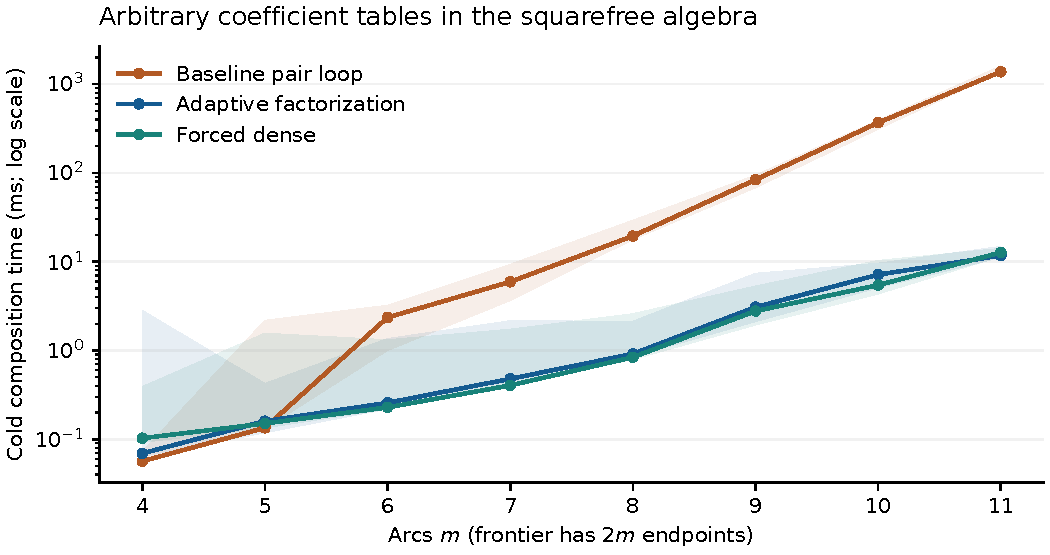
\includegraphics[width=.91\linewidth]{figures/composition_times.pdf}
\caption{The same cold-composition data on a logarithmic time axis.
Points are medians; shaded bands give the observed sample range.
The inputs are valid arbitrary morphisms, with no assertion that these
dense tables arise in the measured knot scans.}
\label{fig:dense}
\end{figure}

At $m=11$, the inputs have 1,019 and 1,014 supported terms. The baseline
populates 1,033,266 monomial-pair memo entries and takes a median
1.378 seconds. The adaptive implementation creates no such pair table and
takes 11.749 milliseconds, a measured factor of 117.28. The small
$m=4,5$ cases show the setup overhead instead. The large dense gain
supports the local algorithmic analysis, but the figure is not a
measurement of 117-fold faster knot recognition. The benchmark inputs
are deliberately general and need not be homogeneous; genuine scanner
entries have the additional structure of Proposition~\ref{prop:grading}.

\subsection{Paired complete scanner workloads}

The full-scanner experiment uses nine fixtures, three composition modes,
and five repetitions, for 135 completed timed scans. Every sample runs in
its own child process, performs one untimed warm-up, and then executes one
timed scan. The legacy process imports the original baseline; the adaptive
and dense processes import the integrated implementation. Each fixture
has one precomputed crossing order and one shape-cache setting, shared by
all modes. Imports, JSON parsing, diagram validation, and order selection
are outside the timed interval. All crossing transfers, cancellations,
rank calculations, and statistics are inside it.

\begin{table}[htbp]
\centering\small
% Generated from archived measurements; do not edit by hand.
\begin{tabular}{lrrrr}
\toprule
Fixture & $n$ & Legacy & Adaptive & Dense \\
\midrule
Trefoil & 3 & 0.388 & 0.566 & 0.464 \\
Figure eight & 4 & 2.373 & 1.153 & 0.737 \\
Conway & 11 & 6.140 & 6.486 & 7.047 \\
Kinoshita--Terasaka & 11 & 8.026 & 9.865 & 11.560 \\
Hard unknot 8 & 8 & 0.863 & 1.339 & 2.424 \\
$T(3,5)$ & 10 & 6.273 & 4.803 & 6.086 \\
$T(3,7)$ & 14 & 11.130 & 10.156 & 12.147 \\
Generated hard unknot 27 & 27 & 16.912 & 25.202 & 33.348 \\
Stress braid5 36 & 36 & 455.644 & 478.966 & 502.907 \\
\bottomrule
\end{tabular}

\caption{Complete scanner medians in milliseconds. Every one of the
135 runs agrees on total rank and the complete homological degree
distribution. These timings use a different, isolated-process protocol
from Table~\ref{tab:quotient}.}
\label{tab:scanner}
\end{table}

The operation counters explain the result more usefully than a selected
speedup number. On all nine fixtures, the adaptive mode selects zero
dense compositions and zero dense transfers. Their maximal frontiers
are at most eight endpoints, where coefficient tables are small. For
example, the 36-crossing stress input reaches 17,694 objects before
elimination and 5,898 afterward, but its maximum frontier is eight.
That workload is dominated by objects, entries, and sparse operations.
The dense asymptotic improvement has no opportunity to dominate there.

Adaptive/legacy median time ratios are 1.056 for Conway, 1.229 for
Kinoshita--Terasaka, 1.490 for the generated 27-crossing hard unknot, and
1.051 for the 36-crossing stress braid. Apparent gains on some small
fixtures are not robust evidence: the figure-eight legacy samples range
from 0.590 to 4.099 milliseconds. These measurements support leaving
\texttt{legacy} as the default. They also identify the next engineering
task: reduce adapter overhead on sparse entries, and find or generate
genuine scan stages whose graded coefficient layers are large enough to
test the new asymptotic regime.

\subsection{Finite-target search and existing filters}

The finite-target comparison uses one untimed warm-up followed by nine
warm repetitions. Search time includes arc extraction, greedy seed-plan
construction, assignment search, and independent certificate replay.
Imports and fixture JSON parsing are excluded. All rows use the same
fixture bytes for the compared procedures. Raw Khovanov time here is a
fallback comparator from this experiment; it must not be mixed with
the isolated full-scanner medians in Table~\ref{tab:scanner}.

\begin{table}[htbp]
\centering\small
% Generated from archived measurements; do not edit by hand.
\begin{tabular}{lrrrrr}
\toprule
Fixture & $b$ & $a$ & $A_5$ seeds & Default & Raw Kh \\
\midrule
Conway & 3 & 57 & 0.781 & 0.645 & 5.516 \\
Kinoshita--Terasaka & 3 & 67 & 0.492 & 0.739 & 6.266 \\
Hard unknot 8$\dagger$ & 2 & 18 & 0.111 & 0.403 & 1.402 \\
$T(3,5)$ & 3 & 35 & 0.549 & 0.155 & 4.281 \\
Stress braid5 36 & 4 & 820 & 7.361 & 0.420 & --- \\
\bottomrule
\end{tabular}

\caption{Warm median milliseconds. $b$ is the discovered seed count and
$a$ the number of complete seed-orbit assignments tried. $\dagger$ marks
an inconclusive $A_5$ search, which has not decided the unknot.
An em dash means that comparator was not measured.}
\label{tab:quotient}
\end{table}

For Conway and Kinoshita--Terasaka, the seed plans use three arcs and find
certificates after 57 and 67 orbit assignments, respectively. Both
certificates have image group of order 60. The seed searches take
0.781 and 0.492 milliseconds, compared with 5.516 and 6.266 milliseconds
for the raw homology fallback in the same protocol. These are useful
fallback savings on those two fixtures. The existing complete recognizer,
however, already rejects both through its Jones stage in about
0.645 and 0.739 milliseconds. The new filter therefore belongs after
the cheap existing obstructions and remains disabled by default.

The 36-crossing stress braid supplies a second caution. The seed search
takes 7.361 milliseconds and finds an image of order 12; the existing
default pipeline takes 0.420 milliseconds. The alternative arc-consistency
solver takes 665.067 milliseconds on that fixture. Search heuristics can
make a large difference even with the same finite target, but beating
another search procedure does not imply beating the recognition pipeline.

For the hard eight-crossing unknot, the seed solver exhausts 18 orbits in
0.111 milliseconds and returns \texttt{INCONCLUSIVE}. Comparing that
time as if it were an unknot decision would be invalid. The separate
$T(3,7)$ control exhausts all 231 seed orbits and likewise stays
inconclusive, as required by the proven $A_5$ obstruction. The constraint
solver also returns inconclusive after 182 search nodes. The archive
includes the certificates for successful cases, the seed plans, and both
exhaustive $T(3,7)$ search records.

\subsection{What the evidence establishes}

The proved local bound, the independently reproduced algebraic identities,
and the dense benchmarks agree. The ordinary full-scanner measurements
show that the missing performance theorem concerns much more than that
primitive. The finite-target backend provides cheap, replayable witnesses
on selected instances, while its negative controls confirm the need for
an exact fallback. No experimental result here establishes a bound on
$b$, $N$, or $Q$ for all knots, a generic advantage from enabling the new
modes, or an unrestricted quasi-polynomial recognizer.

\section{Repository integration and artifact guide}
\label{sec:integration}

\subsection{Compatibility and public interfaces}

The archive contains a self-contained copy of the pinned \texttt{fast/}
package, an exact baseline copy, and a patch with paths relative to the
ProveIt repository root. The implementation needs Python 3.10 or newer
and has no new third-party runtime dependency. The recorded checks use
Python 3.12.14. Matplotlib is needed only to regenerate the research
figure; the figure and generated tables are already included for a
standalone PDF build.

The public scanner options are
\begin{lstlisting}[language=Python]
FastScan(..., composition="legacy")
khovanov_rank(..., composition="legacy")
recognize(..., composition="legacy",
          quotient_max_assignments=0,
          quotient_seconds=0.1)
\end{lstlisting}
The accepted composition modes are \texttt{legacy}, \texttt{adaptive},
and \texttt{dense}. The latter forces the new dense paths while retaining
exact zero, identity, and self-product shortcuts. Nonlegacy modes require
the bits algebra, min-fill cancellation, and self-inverse option where
that option is exposed. Unsupported combinations raise an error. The
implementation does not silently ignore them. Competing worker processes
and factored calls preserve the chosen composition mode, shape-cache
setting, and optional $d^2$ checks.

The finite-target filter is disabled when its assignment budget is zero.
A positive budget applies to complete seed-orbit assignments per examined
summand, across the configured palette. The default cooperative filter
cap is 0.1 seconds; the Python API permits \texttt{None} to remove that
separate cap. A global recognition deadline still limits the filter by
the remaining time. Exhaustion of the filter's own budget records
\texttt{INCONCLUSIVE} and continues. Exhaustion of the global recognition
budget returns \texttt{UNKNOWN}. These distinctions are part of the
public behavior, not merely diagnostic logging.

Example commands, run from \texttt{implementation/fast/}, are
\begin{lstlisting}[language=bash]
python -m fastunknot khovanov examples/conway.json \
  --composition adaptive --check-d2

python -m fastunknot recognize examples/conway.json \
  --no-jones --quotient-max-assignments 5000 \
  --quotient-seconds 0.1

python -m unittest discover -s tests -v
\end{lstlisting}
The second command disables Jones specifically to expose the new
certificate stage on a fixture that the default Jones filter already
handles. It is a demonstration of the fallback, not a recommended change
to filter order.

\subsection{Witness evidence and independent replay}

A successful finite-target search returns method
\texttt{finite-quotient-A5-seeds}. Evidence contains the exact normalized
working \texttt{diagram\_pd}, certificate, checked seed plan, orbit counts,
attempt details, and status. When preprocessing factors a diagram,
the witness belongs to a specified summand and its evidence is stored
with that summand. Existing simplification and factorization correctness
connect that working diagram to the original input. The finite-target
checker itself verifies precisely the PD supplied to it; it does not
claim to replay the earlier Reidemeister or connected-sum transformations.

For an unfactored result whose finite-target stage succeeded, replay is
\begin{lstlisting}[language=Python]
from fastunknot.finite_quotient_check import verify_certificate

evidence = result.evidence["finite_quotient"]
checked = verify_certificate(evidence["diagram_pd"],
                             evidence["certificate"])
assert checked["valid"]
\end{lstlisting}
The supplement also provides a portable helper that replays every
archived certificate against its exact fixture. Keeping explicit
permutations and the precise PD is essential: an image-group order or
an opaque solver state is insufficient evidence by itself.

\subsection{What each directory contains}

\begin{center}
\small
\begin{tabular}{P{.35\linewidth}P{.57\linewidth}}
\toprule
Path & Purpose \\
\midrule
\texttt{article/} & Main TeX file, section sources, generated tables,
vector figure, bibliography, and compiled PDF. \\
\texttt{implementation/fast/} & Runnable package, optional backends,
74-test suite, isolated scanner benchmark, and integration notes. \\
\texttt{baseline/fast/} & Forty source files verified against their
pinned Git blob identities; prior result directories are omitted. \\
\texttt{verification/algebra/} & Portable dense benchmark, scalar
comparison suite, associativity/transfer checks, grading audit, and raw
measurement JSON. \\
\texttt{verification/finite\_quotient/} & Search comparison, certificates,
seed plans, exact fixture bytes, exhaustive negative controls, and replay
helper. \\
\texttt{provenance/} & Repository revisions, baseline blob records,
source normalization details, and validation records. \\
\texttt{tools/} & Table and figure generation, archive verification,
and patch reproduction helpers. \\
\texttt{patches/} & Integration patch against the pinned repository
paths. \\
\bottomrule
\end{tabular}
\end{center}

The top-level README gives exact commands from a freshly extracted
archive. The TeX bibliography is self-contained; no BibTeX or Biber
database download is required. Compiling the main file with ordinary
pdfLaTeX passes resolves the table of contents and cross-references.
The SHA-256 manifest covers the delivered source, data, and PDF files.
The verification helper checks the manifest, the original Git blob
identities, recorded fixture hashes, and the correspondence of the patch
to the supplied baseline and implementation.

\subsection{Merge boundaries}

The intentional edits to existing implementation files are limited to
the scanner selector, public option forwarding and counters, optional
recognizer stage and shared budget, CLI propagation, and the README link.
New modules implement dense composition, finite-target search, and its
separate verifier. The patch includes the new tests and integration
notes. Research measurements and the article may be stored under a new
report directory when integrating the archive.

The patch is concrete and reviewable against the pinned revision. If the
repository has advanced, its changes should be reconciled with the newer
code and the same suite rerun. In particular, report-07 sharing, the
pointed scanner, three-braid specialization, and newer preprocessing
branches are not represented here as an already tested combined release.
The theorem about graded component types applies to the specified exact
sharing construction; implementation and performance of that combined
backend remain a separate, well-defined task.

\section{Further research questions and a proposed programme}
\label{sec:research}

The next stage should be driven by the parameters that remain in the
proved bounds. The following questions are proposed research tasks,
not assertions that their desired answers hold. A useful negative answer
would often be as valuable as a positive one, because it would prevent
investment in a compression invariant that cannot control the algorithm.

\subsection{Priority I: the global structural obstruction}

\begin{question}[Connected components after exact reductions]
\label{q:components}
For which diagram families, or for which residual inputs after the
existing certified filters, can one prove a bound on the largest reduced
connected component size $b$ that makes
$b^2 B_m=O((\log n)^2)$?
\end{question}
This is the most direct missing theorem for the report-07 route. At fixed
frontier, the sufficient condition permits $b=O(\log n)$; it does not
permit arbitrary polynomial growth in $b$. Experiments should record
component sizes, homological spans, matching multiplicities, dot-degree
layers, and weights at every stage. Families designed to resist
connected-sum factorization and elementary simplification are especially
valuable. If $b$ grows too quickly even at fixed width, determine whether
the growth is forced under every admissible cancellation order, or is
an artifact of the chosen pivot policy. A proof of such an obstruction
would redirect the programme toward stronger equivalence relations.

\begin{question}[Compression beyond identical serialized components]
Can a constructive chain-homotopy normalization replace large connected
components by a bounded description while preserving the recognition
criterion and efficient future crossing updates?
\end{question}
Exact component sharing only merges identical keys. It does not perform
arbitrary changes of basis or discover every homotopy equivalence.
Candidate descriptions include graded module decompositions, interval
structures in restricted categories, and presentations over small
endomorphism algebras. Each proposal must specify the allowed basis
changes, provide an algorithm to compute the description, and bound
composition after a crossing is added. Merely knowing that equivalent
complexes have a small representative is insufficient if finding or
updating it requires enumerating exponentially many bases. Test the
proposal first on the known multiplicity families and on connected
examples that cannot be removed by visible sum decomposition.

\begin{question}[Crossing order optimized for the real cost]
Can crossing orders be constructed with controlled
$w+\log(N+2)$, or controlled $b^2 B_{w/2}$, rather than with small
frontier alone?
\end{question}
A frontier objective sees only one part of the resource envelope.
The stress fixture in Table~\ref{tab:scanner} has a small frontier and
thousands of surviving objects. A useful ordering certificate would
explain why its chosen local pieces have bounded component growth, not
just count exposed endpoints. Investigate separator decompositions with
independent frontier components, preserving a certified disk order only
where that order actually exists. Any Catalan estimate must carry the
topological ordering certificate that makes it valid. Approximation or
heuristic ordering results should charge the time spent finding the order.

\begin{question}[A completeness theorem for a portfolio]
Can one prove that every diagram either admits a cheap structural or
finite-target certificate, or enters the homology backend with parameters
satisfying a quasi-polynomial bound?
\end{question}
This formulation respects the difference between complete homology
calculation and unknot recognition. The full invariant can be expensive
even when a simple certificate already decides the knot. A successful
theorem would describe a finite or effectively generated set of cases,
prove coverage, and bound how the appropriate case is found. It must also
account for unknot inputs, where knottedness filters cannot help. The
current three-braid, homogeneous-diagram, connected-sum, Alexander,
Jones, and finite-target stages are concrete candidates for parts of
such a partition, but present experiments do not prove that their
residual class has small $b$ or small width.

\subsection{Priority II: exploit the grading in the representation}

\begin{question}[Rank-layer coefficient storage]
Can a homogeneous $k$-circle coefficient of dot degree $d$ be stored
and manipulated in time near $\binom{k}{d}$, with no full $2^k$ table
allocated during contraction or output reconstruction?
\end{question}
Theorem~\ref{thm:homogeneous} reduces the transform arithmetic, while
Theorem~\ref{thm:types} reduces the number of possible coefficients.
The current implementation still allocates subset-indexed tables.
Combinatorial ranking of fixed-cardinality subsets, restricted zeta
transforms, or sparse-to-layer conversions might realize the counting
gain in memory as well. The challenge is closure: identifying input
variables can kill terms and combine them by parity, and the output map
has nontrivial block structure. A valid result must cover those maps,
not just multiplication of two already indexed middle layers. Compare
the resulting cost with both input and output layer sizes.

\begin{question}[A grading-aware scanner interface]
Should the quantum shifts be stored explicitly to eliminate impossible
entries earlier, restrict pivot search, and specialize every genuine
cancellable unit to $1$?
\end{question}
The proof shows that the information is recoverable; the current audit
reconstructs it separately. An explicit grading can reject incompatible
matrix entries before compiling a surface plan and can provide a useful
internal consistency check. Measure whether the saved work exceeds the
cost of maintaining shifts and layer metadata. The interface must retain
the generic algebra fallback for clients that intentionally supply
inhomogeneous morphisms. A separate graded object type is preferable to
silently assuming homogeneity from the packed coefficient's shape.

\begin{question}[Remove sparse-case adapter overhead]
Can the implementation preserve the baseline cost on small or sparse
entries while retaining the proved dense envelope?
\end{question}
This is a high-confidence engineering task suggested directly by the
paired timings. A fixed small-frontier dispatch to the original primitive
preserves the asymptotic theorem, because its cutoff is constant.
More general dispatch must also charge output expansion and large-integer
updates; a support-only estimate can be misleading. Profile plan lookup,
support extraction, homogeneity detection, byte conversion, and cache
reuse separately. Promote a new default only after paired scans on both
ordinary inputs and genuinely dense graded stages demonstrate a useful
tradeoff. Retain raw distributions rather than optimizing one selected
median on a noisy machine.

\begin{question}[What dense entries can actually occur?]
Is there an explicit knot-diagram family producing large, dense
homogeneous differential entries after the prescribed cancellations,
and can their density be predicted from topology?
\end{question}
The arbitrary-algebra family in Section~\ref{sec:convolution} proves a
local worst-case improvement. It does not supply a knot family realizing
that local worst case. A useful construction would preserve exact stage
data and provide a proof of its coefficient support, rather than merely
an opaque slow example. Conversely, a theorem limiting support density
in all relevant surviving complexes might make a different sparse
algorithm the right asymptotic target. This question connects the
coefficient theorem to end-to-end usefulness.

\begin{question}[Other characteristics and integral coefficients]
How far does the plan factorization extend with controlled bit complexity
over odd finite fields or over the integers?
\end{question}
Ranked subset convolution works over much more general coefficient rings
than $\F$~\cite{bhkk}. The geometric specialization needs separate
attention: the handle multiplier $2x$ no longer vanishes in odd
characteristic, integer signs must be consistent, and integer coefficient
growth must be bounded. A graded unit may be a nonzero scalar requiring
inversion, rather than the unique scalar $1$. An extension should specify
the exact Frobenius algebra, prove the new component evaluation formula,
and charge coefficient bit lengths. It should not simply reuse the
characteristic-two positive-genus shortcut.

\subsection{Priority III: bounded witnesses and target selection}

\begin{question}[Constructive seed-plan quality]
Can the greedy $O(n^3)$ seed-plan construction be replaced by a faster
dependency-closure algorithm, with a useful approximation or structural
bound on the resulting seed count?
\end{question}
For fixed targets, lowering $b$ by one saves an exponential factor in
the search parameter, while a smaller planning constant matters for
sub-millisecond fixtures. Maintain the crossing dependencies exposed by
each newly colored arc, and reuse closure information between candidate
seeds. Prove the setup cost of this reuse and keep the final plan
independently checkable. The equality between the minimum Wirtinger
number over diagrams and bridge number~\cite{blair} is a structural
guide; it does not make minimum-seed search on an arbitrary presented
diagram free.

\begin{question}[Adaptive finite targets with a completeness bound]
Can target groups or quandles be constructed from a diagram so that
every nontrivial residual knot has a witness with
$b\log(q+1)=O((\log n)^2)$, and both target construction and witness
search fit the same budget?
\end{question}
The palette obstruction rules out a universal bounded palette. The
NP-completeness result for fixed-target coloring~\cite{kuperbergsamperton}
also prevents a casual inference from a small target to an easy search
for every diagram. A constructive target-selection theorem would need
to exploit special structure or permit a different obstruction when
a target search is difficult. Count the target description, conjugation
table or on-demand operation cost, seed plan, and proof of nonconstancy.
Do not replace all these requirements by an existence theorem for some
finite nonabelian quotient.

\begin{question}[Sharp detecting-quandle size for determinant-one torus knots]
What is the smallest size $q(p)$ of a finite quandle that nontrivially
colors $T(3,p)$, for prime $p>3$? Can the lower bound $q(p)\geq p$
be improved, and can one give explicit detecting targets with comparable
upper bounds?
\end{question}
The proof uses the exponent of the inner group and works for nonfaithful
and disconnected quandles. It does not show that a size-$p$ target exists.
Study conjugacy classes in explicit finite quotients of the torus group,
and compare their class size with the size of the entire group. Distinguish
the number of quandle elements from the encoding length of a succinct
group. Determinant one already removes familiar affine-coloring routes;
the non-affine constructions discussed by Fish, Lisitsa, and
Stanovsk\'y~\cite{fish} give relevant precedent. Small computational
classifications could suggest a sharper theorem, but should not be
advertised as a bound for untested primes.

\subsection{Priority IV: alternate routes to a global theorem}

\begin{question}[Detecting slices with a completeness guarantee]
For which broad knot families does nontrivial reduced Khovanov homology
necessarily appear within a provably shallow extremal homological band?
\end{question}
Combine a genuine detection theorem with the prescribed nice-scan
construction of Kelom\"aki and Sch\"utz~\cite{kelomaki}. For the
displayed slice envelope, $g=O((\log n)^2)$ and $k=O(\log n)$ would
fit the stronger $n^{O(\log n)}$ scale, provided the scan is constructed
within that cost. A fast slice without a theorem locating the required
homology is only a partial obstruction. Also quantify what happens when
the useful grading range is specified in normalized knot-theoretic
degrees rather than unshifted cube degrees; crossing-sign shifts must
be handled explicitly.

\begin{question}[A complete hierarchy cost ledger]
Can the hierarchy approach be organized into explicit compressed data
structures for which every visit, cut, normalization, and violating-disc
step has a proved bit bound?
\end{question}
Lackenby's bound $L(g+1)^L$ has logarithm
$O(\log(L+1)+L\log(g+1))$~\cite{lackenby2026}. Thus
$L\log(g+1)=O((\log n)^2)$ is a natural target for the stronger
scale in this project, while $O((\log n)^3)$ would still yield the
broader quasi-polynomial scale announced in the 2021 handout.
If $g$ is polynomial in $n$, these correspond to hierarchy lengths of
order $\log n$ and $(\log n)^2$, respectively. These statements bound
visit counts only. Compressed surface coordinates can encode extremely
large geometric objects, so naive expansion during a cut would destroy
the argument. The normal-curve algorithms in~\cite{lackenbycurves}
suggest useful primitives, but the full ledger and construction theorem
must be written and proved.

\begin{question}[Certificates for the algebraic reduction itself]
Can every crossing extension and cancellation emit a compact reduction
certificate whose verifier is substantially simpler than the optimized
scanner?
\end{question}
The finite-target work demonstrates the practical value of a search and
verifier separation. For homological reduction, record the pivot,
inclusion and projection maps, and the relevant chain-homotopy identity.
The challenge is certificate size: an explicit transcript can be as
large as the computation. Investigate compressed transcripts with
deterministically replayable local claims, and state whether verification
requires the same coefficient tables. A formalization can begin with the
squarefree-algebra factorization, ranked convolution, and scalar
cancellation identity, while clearly treating the topological
unknot-detection theorem as a separately cited assumption.

\subsection{Concrete milestones}

The next release can have measurable goals without pretending to settle
the global problem immediately.
\begin{enumerate}
\item \textbf{Instrument the surviving structure.} Merge grading metadata
with report-07 sharing in an isolated branch, recording $m$, $b$, $N$,
component weights, and dot-degree distributions. First reproduce the
existing exact outputs; then publish the component-growth data.
\item \textbf{Improve ordinary workloads.} Add a constant-frontier legacy
dispatch and a measured cache policy, while preserving the proved
coefficient envelope. Require paired ordinary scans and genuine graded
dense cases before changing defaults.
\item \textbf{Prove one nontrivial structural family theorem.} Choose a
family after the existing certified filters and prove its actual
component-size or homotopy-description bound. A theorem with an explicit
construction is more informative than a larger table of favorable
timings.
\item \textbf{Publish a falsifiable global route.} State exactly which
structural dichotomy or hierarchy construction would imply the desired
bound, and keep every unproved lemma visible. Search deliberately for
counterexamples to those lemmas before expanding the implementation.
\end{enumerate}

The present continuation has made coefficient operations essentially
linear in their explicit table size up to polynomial frontier factors,
and it has improved the available counting argument through a recovered
grading. The proposed programme now concentrates on the amount and
structure of data that the algorithm must construct. That is the point
at which the quasi-polynomial objective will be decided.

% Primary-source metadata and theorem locators checked on 7 October 2026.
% Self-contained bibliography: no BibTeX or Biber invocation is required.
\begin{thebibliography}{99}
\addcontentsline{toc}{section}{References}

\bibitem{barnatan}
Dror Bar-Natan,
\emph{Fast Khovanov homology computations},
Journal of Knot Theory and Its Ramifications
\textbf{16} (2007), no.~3, 243--255.
\href{https://arxiv.org/abs/math/0606318v1}{arXiv:math/0606318v1}.
\href{https://www.math.utoronto.ca/~drorbn/papers/FastKh/FastKh.pdf}{Author's version of 20 May 2007}.
Section~3 gives the local dotted relations; Lemmas~4.1--4.2 give
delooping and abstract Gaussian elimination.

\bibitem{barnatancobordisms}
Dror Bar-Natan,
\emph{Khovanov's homology for tangles and cobordisms},
Geometry \& Topology \textbf{9} (2005), 1443--1499.
\href{https://doi.org/10.2140/gt.2005.9.1443}{doi:10.2140/gt.2005.9.1443}.
\href{https://arxiv.org/abs/math/0410495v2}{arXiv:math/0410495v2}.
This supplies the formal tangle/cobordism framework underlying the local
algorithm; see Section~11.2 for the dotted specialization.

\bibitem{bhkk}
Andreas Bj\"orklund, Thore Husfeldt, Petteri Kaski, and Mikko Koivisto,
\emph{Fourier meets M\"obius: fast subset convolution},
in Proceedings of the 39th Annual ACM Symposium on Theory of Computing
(STOC 2007), ACM, 2007, 67--74.
\href{https://doi.org/10.1145/1250790.1250801}{doi:10.1145/1250790.1250801}.
\href{https://arxiv.org/abs/cs/0611101v1}{arXiv:cs/0611101v1}.
The algorithm computes subset convolution in $O(r^2 2^r)$ ring operations.

\bibitem{blair}
Ryan Blair, Alexandra Kjuchukova, Roman Velazquez, and Paul Villanueva,
\emph{Wirtinger systems of generators of knot groups},
Communications in Analysis and Geometry
\textbf{28} (2020), no.~2, 243--262.
\href{https://doi.org/10.4310/CAG.2020.v28.n2.a2}{doi:10.4310/CAG.2020.v28.n2.a2}.
\href{https://arxiv.org/abs/1705.03108v1}{arXiv:1705.03108v1}.
The introduction defines seed strands and diagrammatic propagation;
Theorem~1.3 identifies the minimum over diagrams with bridge number.

\bibitem{clark}
W.~Edwin Clark, Mohamed Elhamdadi, Masahico Saito, and Timothy Yeatman,
\emph{Quandle colorings of knots and applications},
Journal of Knot Theory and Its Ramifications
\textbf{23} (2014), no.~6, article 1450035, 29~pp.
\href{https://doi.org/10.1142/S0218216514500357}{doi:10.1142/S0218216514500357}.
\href{https://arxiv.org/abs/1312.3307v2}{arXiv:1312.3307v2}.
Appendix~D describes the normalization fixing one color in a connected
quandle braid-coloring search.

\bibitem{fish}
Andrew Fish, Alexei Lisitsa, and David Stanovsk\'y,
\emph{A combinatorial approach to knot recognition},
preprint, 25 May 2015.
\href{https://arxiv.org/abs/1505.06595v1}{arXiv:1505.06595v1}.
Theorems~2--3 discuss finite-quandle detection and the relation between
finite affine colorings and the Alexander polynomial; the paper also
describes SAT-based coloring search.

\bibitem{kelomaki}
Tuomas Kelom\"aki and Dirk Sch\"utz,
\emph{On computational complexity of Khovanov homology},
preprint, 5 January 2026, 30~pp.
\href{https://arxiv.org/abs/2601.02119v1}{arXiv:2601.02119v1}.
Theorems~1.2--1.4 distinguish exponential scanning examples, the specialized
three-braid algorithm, and extremal homological bands. Proposition~5.1 and
Lemma~5.5 give the supplied-nice-scan bounds used in the parameter discussion.

\bibitem{kronheimer}
Peter B.~Kronheimer and Tomasz S.~Mrowka,
\emph{Khovanov homology is an unknot-detector},
Publications Math\'ematiques de l'IH\'ES
\textbf{113} (2011), 97--208.
\href{https://doi.org/10.1007/s10240-010-0030-y}{doi:10.1007/s10240-010-0030-y}.
\href{https://arxiv.org/abs/1005.4346v1}{arXiv:1005.4346v1}.
Corollary~1.3, Proposition~1.4, and the discussion in the introduction give
reduced rational rank greater than one for every nontrivial knot. The
universal coefficient theorem then gives the required lower bound over
$\mathbb F_2$.

\bibitem{kuperbergsamperton}
Greg Kuperberg and Eric Samperton,
\emph{Coloring invariants of knots and links are often intractable},
Algebraic \& Geometric Topology
\textbf{21} (2021), 1479--1510.
\href{https://doi.org/10.2140/agt.2021.21.1479}{doi:10.2140/agt.2021.21.1479}.
\href{https://arxiv.org/abs/1907.05981v1}{arXiv:1907.05981v1}.
Theorem~1.1 gives the counting hardness result; Corollary~1.2 gives
NP-completeness of nonconstant coloring for a fixed nontrivial conjugacy
class in a fixed finite nonabelian simple group.

\bibitem{lackenbytalk}
Marc Lackenby,
\emph{Unknot recognition in quasi-polynomial time},
Oxford topology seminar handout, March 2021, 34~pp.
\href{https://people.maths.ox.ac.uk/lackenby/quasipolynomial-talk-oxford-compressed.pdf}{Author's seminar handout}.
The announced $2^{O((\log n)^3)}$ bound appears on slide~7;
the proposed speed-up ingredients are summarized from slide~25 onward.
This citation records the announcement and does not turn the slides into
a complete published complexity proof.

\bibitem{lackenby2026}
Marc Lackenby,
\emph{Incompressible surfaces, hierarchies and unknot recognition},
preprint, 25 July 2026, 54~pp.
\href{https://arxiv.org/abs/2607.23350v1}{arXiv:2607.23350v1}.
\href{https://arxiv.org/html/2607.23350v1}{Version-pinned full text}.
Proposition~9.1 gives the $L(g+1)^L$ step-visit bound. Theorem~14.1
concerns polynomially encoded and verifiable essential hierarchies.
The introduction leaves additional running-time improvements to future work.

\bibitem{lackenbycurves}
Marc Lackenby,
\emph{Some fast algorithms for curves in surfaces},
Discrete \& Computational Geometry, published online 21 April 2026.
\href{https://doi.org/10.1007/s00454-026-00845-7}{doi:10.1007/s00454-026-00845-7}.
\href{https://arxiv.org/abs/2401.16056}{arXiv:2401.16056}.
\href{https://people.maths.ox.ac.uk/lackenby/AlgorithmsSurfaces13jan26.pdf}{Author's version of 13 January 2026}.
The compressed normal-curve primitives are relevant to the geometric
research programme, without supplying a complete hierarchy-search bound.

\bibitem{openai}
OpenAI,
\emph{math: mathematical manuscripts and catalogue},
repository snapshot at commit
\texttt{adc7f1241b42e322a6451854ab7e4b4c146bf78a},
accessed 7 October 2026.
\href{https://github.com/openai/math/tree/adc7f1241b42e322a6451854ab7e4b4c146bf78a}{Pinned repository}.
Only the README and catalogue were used for the applicability audit;
no result in this article relies on an unchecked manuscript from the collection.

\bibitem{proveit}
Vladimir Reshetnikov,
\emph{ProveIt: Topology/UnknotRecognition},
software and research repository, source snapshot at commit
\texttt{ca61a1a5f967999d778d6efd7c882e77a2eb379d},
accessed 7 October 2026.
\href{https://github.com/VladimirReshetnikov/ProveIt/tree/ca61a1a5f967999d778d6efd7c882e77a2eb379d/Topology/UnknotRecognition}{Pinned project source}.
The present integration patch targets this snapshot's \texttt{fast/} subtree.

\bibitem{report07}
ProveIt research continuation,
\emph{Unknot recognition by structural certificates and compressed chain
complexes: exact improvements and a finite-type route towards
quasi-polynomial time},
research report~07, 7 October 2026.
\href{https://github.com/VladimirReshetnikov/ProveIt/tree/ca61a1a5f967999d778d6efd7c882e77a2eb379d/Topology/UnknotRecognition/reports/07}{Report and accompanying implementation in the pinned repository}.
This is a project research artifact, not a journal publication. Its own
implementation baseline is identified as commit
\texttt{4e6fe879e5238ec0b134b6d33fdca0b8c7c1c711}.

\bibitem{shumakovitch}
Alexander N.~Shumakovitch,
\emph{Torsion of Khovanov homology},
Fundamenta Mathematicae \textbf{225} (2014), 343--364.
\href{https://doi.org/10.4064/fm225-1-16}{doi:10.4064/fm225-1-16}.
\href{https://arxiv.org/abs/math/0405474v2}{arXiv:math/0405474v2},
revised 19 June 2018 to match the published version.
Corollary~3.2.C gives the direct-sum relation between unreduced and reduced
Khovanov homology over $\mathbb F_2$, with quantum shifts $\pm1$.

\end{thebibliography}

\end{document}
